\documentclass[10pt]{article}
\usepackage{graphicx,tabularx,array,geometry,tikz,pgfplots,amsmath,bbding,framed,enumitem,graphicx,wrapfig,multicol,listings,empheq,caption,float}
\usepackage{color} %red, green, blue, yellow, cyan, magenta, black, white
\definecolor{mygreen}{RGB}{28,172,0} % color values Red, Green, Blue
\definecolor{mylilas}{RGB}{170,55,241}
\usepackage[makeroom]{cancel}
\usepackage[utf8]{inputenc}
\usepackage[english]{babel}
\usepackage[nottoc]{tocbibind}

\setlength{\parskip}{2ex} %--skip lines between paragraphs
\setlength{\parindent}{0pt} %--don't indent paragraphs
\lstset{language=Matlab,%
  %basicstyle=\color{red},
  breaklines=true,%
  morekeywords={matlab2tikz},
  keywordstyle=\color{blue},%
  morekeywords=[2]{1}, keywordstyle=[2]{\color{black}},
  identifierstyle=\color{black},%
  stringstyle=\color{mylilas},
  commentstyle=\color{mygreen},%
  showstringspaces=false,%without this there will be a symbol in the places where there is a space
  numbers=left,%
  numberstyle={\tiny \color{black}},% size of the numbers
  numbersep=9pt, % this defines how far the numbers are from the text
  emph=[1]{for,end,break},emphstyle=[1]\color{red}, %some words to emphasise
  %emph=[2]{word1,word2}, emphstyle=[2]{style},    
}
\geometry{
 total={210mm,297mm},
 left=22mm,
 right=22mm,
 top=25mm,
 bottom=25mm,
 }
 \pgfplotsset{compat=1.12}
%-- Commands for header
\newcommand*\widefbox[1]{\fbox{\hspace{2em}#1\hspace{2em}}}
\renewcommand{\title}[1]{\textbf{#1}\\}
\renewcommand{\line}{\begin{tabularx}{\textwidth}{X>{\raggedleft}X}\hline\\\end{tabularx}\\[-0.5cm]}
\newcommand{\leftright}[2]{\begin{tabularx}{\textwidth}{X>{\raggedleft}X}#1%
\end{tabularx}\\[-0.5cm]}

%\linespread{2} %-- Uncomment for Double Space
\begin{document}

%\title{Final 22.212 Report\qquad Amelia Trainer }
%\line\\
%\leftright{\today}{ }%-- left and right positions in the header
%~\par

\begin{center}\section*{Identifying the effect that changing $\delta$ functions to triangles has on $S(\alpha,\beta)$, for H in H$_2$O}

  Amelia Trainer \\
  \today
\end{center}

\begin{multicols}{2}
%\section{Introduction}
\subsection*{NJOY2016 Test09 Spectrum}

  Fig.~\ref{fig:waterPhonon} contains the phonon spectrum that NJOY2016 uses in their Test09 documentation. This test is used as a simplified model for the H in H$_2$O interactions. 
            \begin{figure}[H]
              \begin{center}
              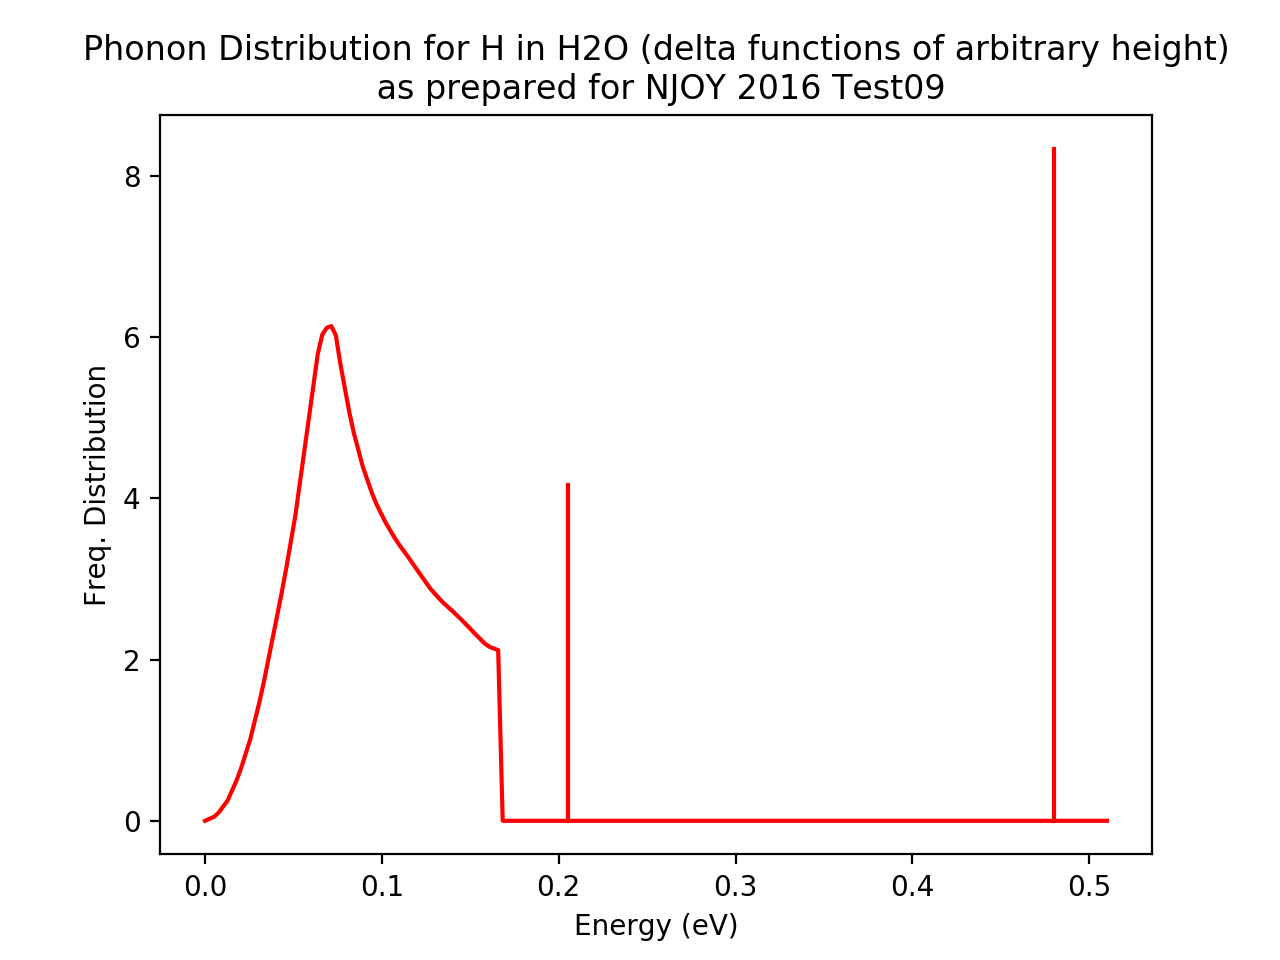
\includegraphics[scale=0.5]{waterPhononDist}
                \caption{NJOY 2016 contains Test09, a simplified model for H in H$_2$O. Part of this model is a frequency distribution, which is shown above. It contains a continuous contribution, shown on the lower energy region, and two $\delta$ functions to approximate the behavior for higher energies.}
              \label{fig:waterPhonon}
              \end{center}
            \end{figure}

The phonon distribution for NJOY2016 Test09 has a grid spacing 0.00255 eV, with the $\delta$ functions located at 0.205 and 0.48 eV. The continuous part is weighted to 0.5, and the two delta functions are weighted to 0.166667 and 0.333333 eV, respectively. Thus these three components have the frequency distribution to be weighted to 1.0. The $\delta$ function properties are also listed in Table 1. The real Test09 also has a translational contribution, which we choose to remove and ignore for this discussion.

\begin{center}
\begin{tabular}{ |c|c| }\hline
 Energy (eV)& Weighting\\\hline
 0.205& 0.166667\\\hline
 0.480 & 0.333333 \\\hline
\end{tabular}\\[1ex]
Table 1. Energies and weights of the two $\delta$ functions that appear in NJOY2016 Test09's phonon spectrum.
\end{center}
  
  \subsection*{Problem Specification}
  We approximate the delta functions to be triangles of various widths. This is shown in Fig.~\ref{fig:waterPhononTriangle}. The continuous description spans from 0 eV to 0.17 eV.


            \begin{figure}[H]
              \begin{center}
              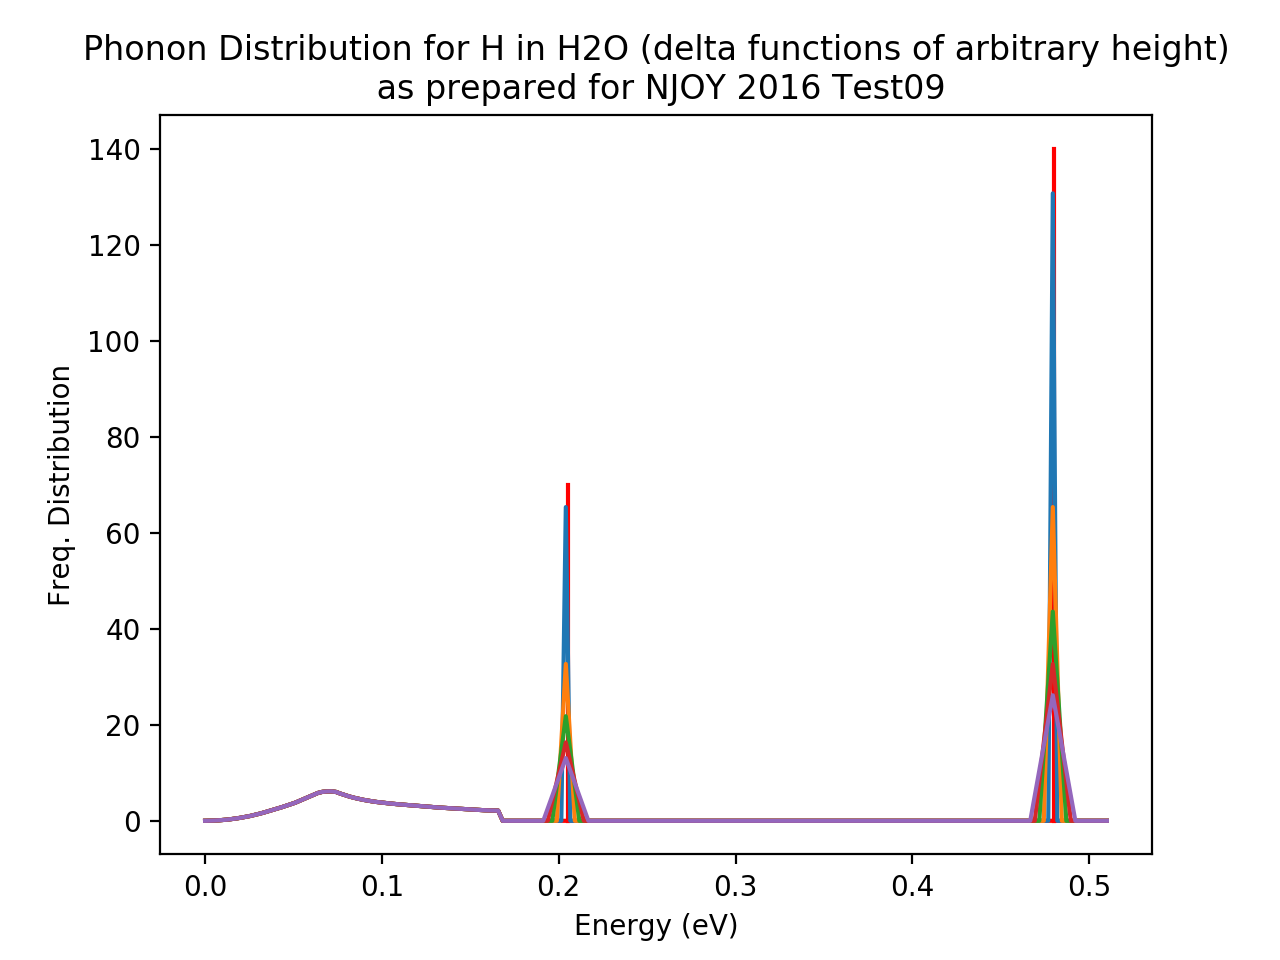
\includegraphics[scale=0.5]{waterPhononDistTriangles}
                \caption{}
              \label{fig:waterPhononTriangle}
              \end{center}
            \end{figure}

  Let's zoom into the 0.205 eV $\delta$ function, shown in Fig.~\ref{fig:waterPhononTriangleZoomed}. The blue triangle has a total width of 2 grid spacings, the yellow has a total width of 4 grid spacings, etc. They are constructed to preserve the relative weigthing between the lower energy continuous piece, and the individual $\delta$ functions in the higher energy region.\par
  
  Note that since the triangle approximations are forced to stay on the predetermined phonon grid with spacing 0.00255, the triangles used do not exactly line up with the actual $\delta$ functions that are provided in the Test09 documentation (i.e. the red line in Fig.~\ref{waterPhononTriangleZoomed} does not fall in the center of the triangles). Thus, for the purposes of this discussion, we'll artificially shift over the $\delta$ functions, so that they can line up with the 0.00255 eV grid. We will no longer consider the $\delta$ functions to be located at 0.205 and 0.48 eV, but rather 0.204 and 0.4794 eV, respectively. These values, which are used for the rest of this discussion, are provided in Table 2.

\begin{center}
\begin{tabular}{ |c|c| }\hline
 Energy (eV)& Weighting\\\hline
 0.204& 0.166667\\\hline
 0.4794 & 0.333333 \\\hline
\end{tabular}\\[1ex]
Table 2. Energies and weights of the two $\delta$ functions that are used for the rest of this discussion. They were chosen so as to line up on the predetermined freq. distribution grid, which has spacing of 0.00255 eV.
\end{center}
 
            \begin{figure}[H]
              \begin{center}
              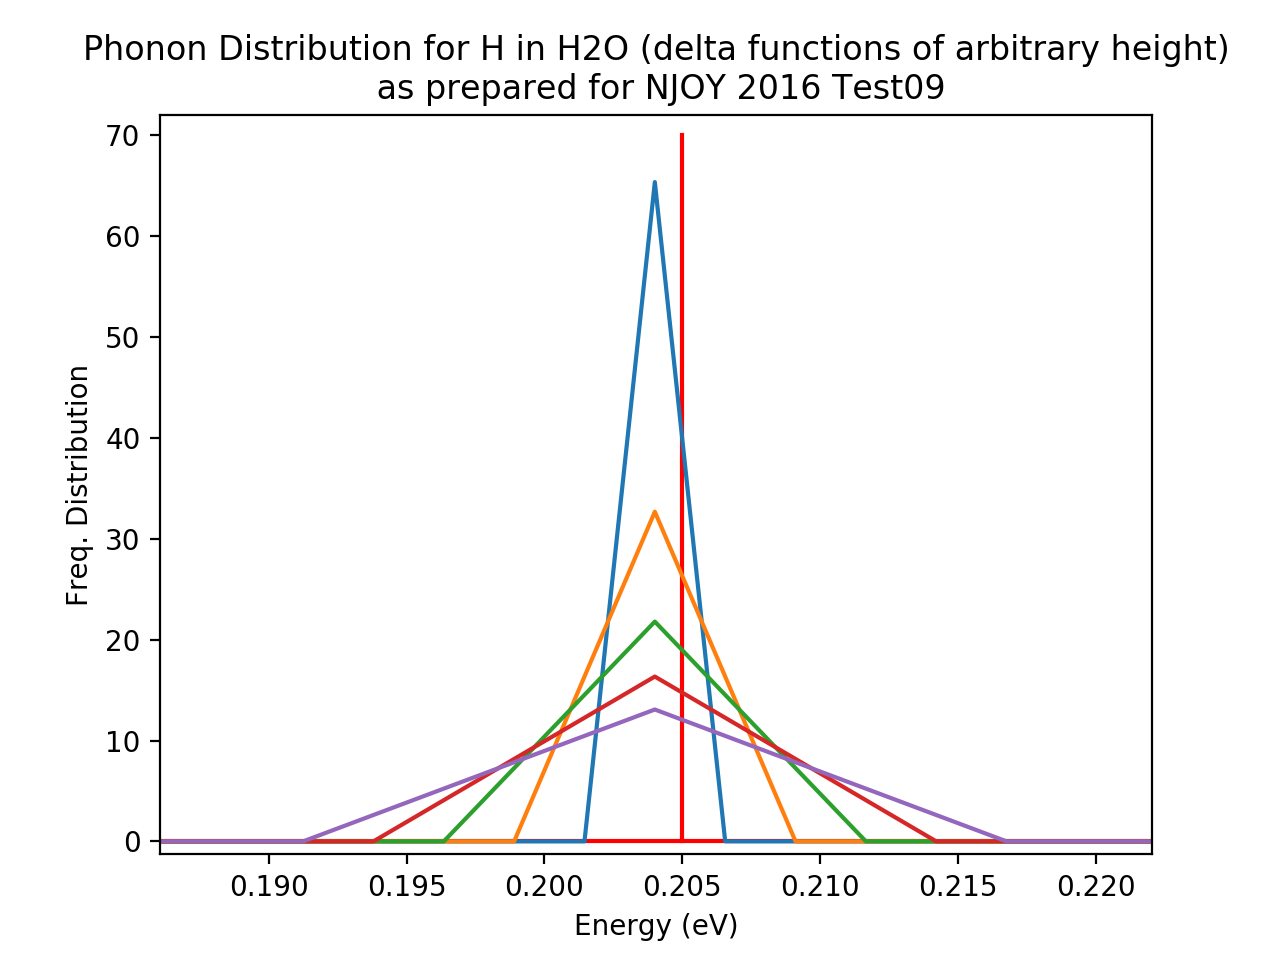
\includegraphics[scale=0.5]{waterPhononDistTrianglesZoomed}
                \caption{This is a zoomed in version of Fig.~\ref{fig:waterPhononTriangle}, where we focus in on the 0.204 eV $\delta$ function. The red line represents the $\delta$ function that is defined in the NJOY2016 Test09 statement, while the other colors represent triangles that are being used to approximate this $\delta$ function. The triangles have width $2\times\Delta E,4\times\Delta E,6\times\Delta E,...$, where $\Delta E=0.00255$~eV. The important thing to notice is that the $\delta$ function doesn't line up with the triangles (because the triangles are restricted to a 0.00255 eV grid), so we're brought to adjust the $\delta$ function specifications from those in Table 1, to those in Table 2.}
              
              \label{fig:waterPhononTriangleZoomed}
              \end{center}
            \end{figure}


\subsection*{Results: Thin Triangle vs. $\delta$ Func.}
We use the phonon distributions generated earlier as input for NJOY, and generate resultant $S(\alpha,\beta)$ grids. We consider a phonon distribution with $\delta$ functions describing the higher energy region (with the energies and weights that are presented in Table 2), alongside a phonon distribution with thin triangles approximating the $\delta$ functions. The triangles used to approximate the $\delta$ functions have a total width of two spaces, or $2\times0.00255=0.0051$~eV.

            \begin{figure}[H]
              \begin{center}
              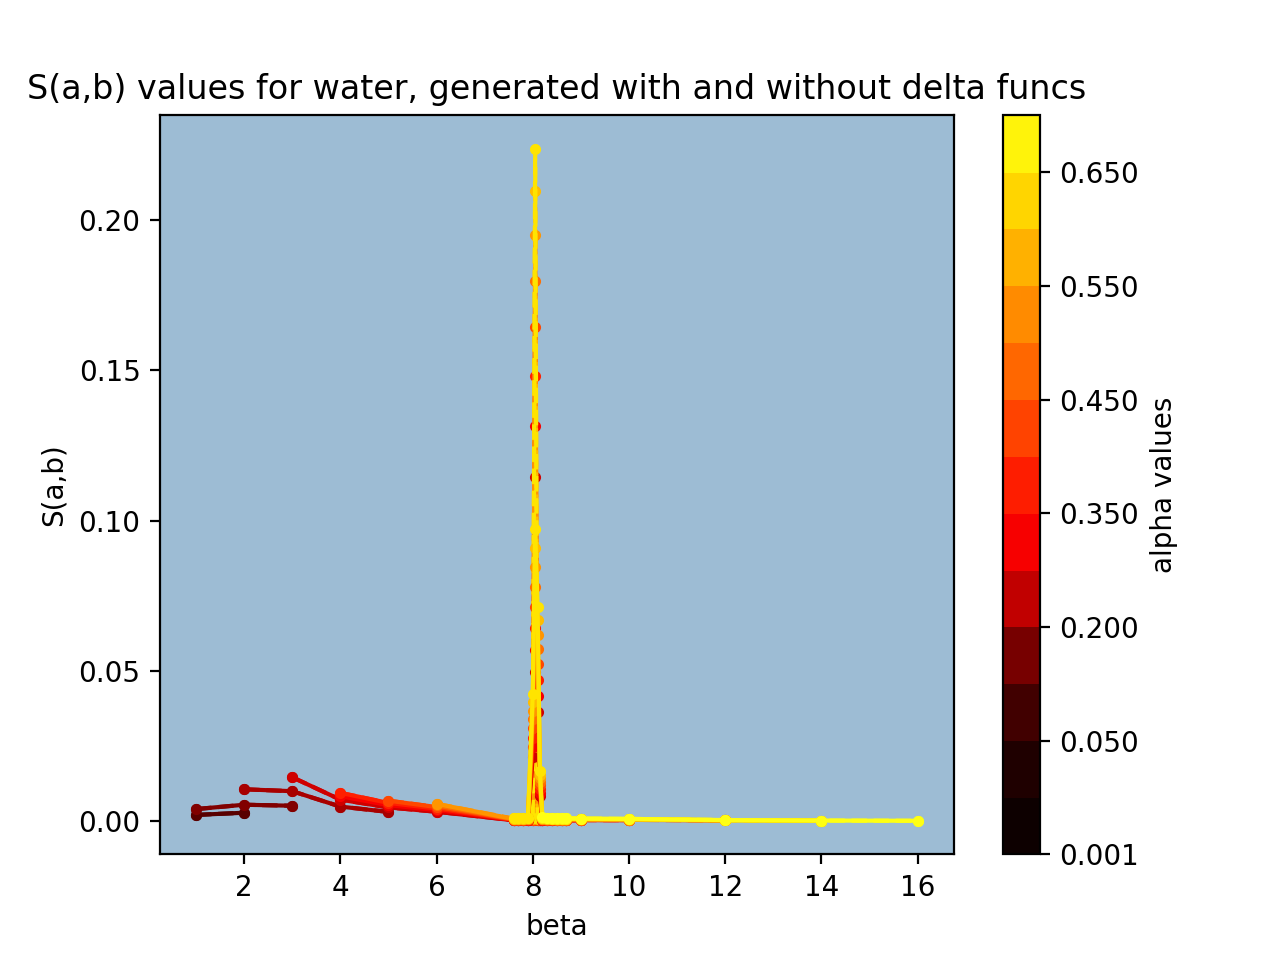
\includegraphics[scale=0.6]{sab_thinTriangle_and_delta_all_AB}
                \caption{NJOY is used to generate the above plots, where we plot $S(\alpha,\beta)$ against $\beta$, for various $\alpha$ values. Note that since not all $\alpha$ values are compatible with all $\beta$ values, we have discrete line sort of behavior, especially for the low $\beta$ region. }
              \label{fig:sabThinTriangleAllAB}
              \end{center}
            \end{figure}



            \begin{figure}[H]
              \begin{center}
              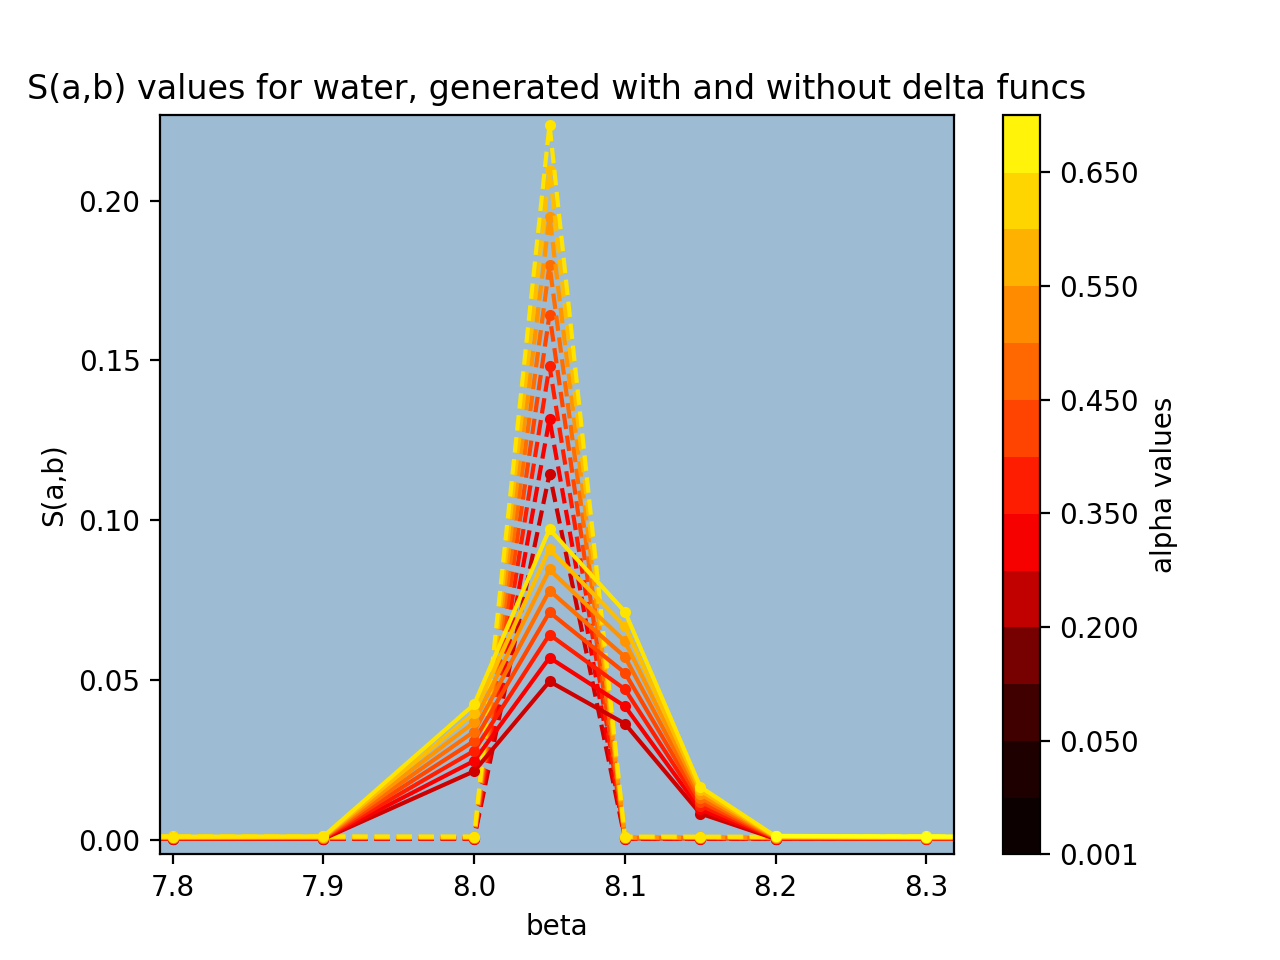
\includegraphics[scale=0.6]{sab_thinTriangle_and_delta_all_AB_Zoomed}
                \caption{This is the same as Fig.~\ref{fig:sabThinTriangleAllAB}, except we zoom in on the peak near $\beta\approx8.05$. The dotted lines correspond to the values produced by NJOY using $\delta$ functions in the phonon distribution, while the solid lines correspond to those $\delta$ functions being approximated by a thin triangle.}
              \label{fig:sabThinTriangleAllABZoomed}
              \end{center}
            \end{figure}


            Let's look at Fig.~\ref{fig:sabThinTriangleAllABZoomed}, which is a zoomed-in version of Fig.~\ref{fig:sabThinTriangleAllAB}. It shows the $S(\alpha,\beta)$ values that were generated using NJOY for H in H$_2$O, wusing the $\delta$ function phonon distribution (dotted lines) and the triangle approximation to $\delta$ functions (solid lines). Note that $S(\alpha,\beta)$ grid that uses the triangle approximation for its higher energy peaks has more of a smear than the one that uses $\delta$ functions, which seems pretty reasonable.

            \begin{figure}[H]
              \begin{center}
              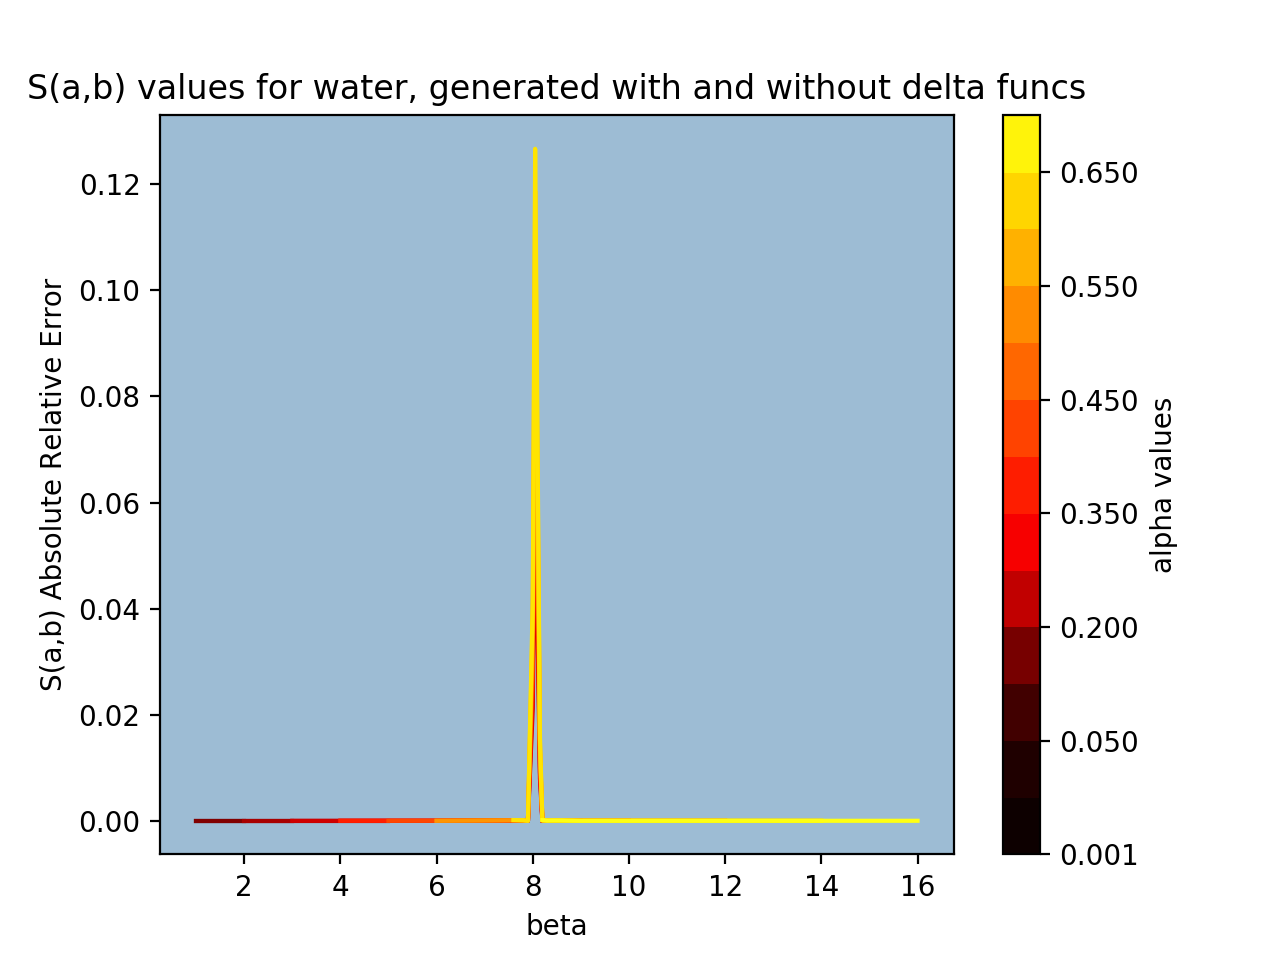
\includegraphics[scale=0.6]{sab_thinTriangle_error}
                \caption{This is the absolute relative error between the $S(\alpha,\beta)$ produced using $\delta$ functions and $S(\alpha,\beta)$ produced using a thin (width = 2 spaces) triangle. Note that the error is very small away from the $\beta\approx8.05$ peak. }
              \label{fig:sabThinTriangleError}
              \end{center}
            \end{figure}




\subsection*{Results: Triangles of Various Widths vs. $\delta$ Func.}

            \begin{figure}[H]
              \begin{center}
              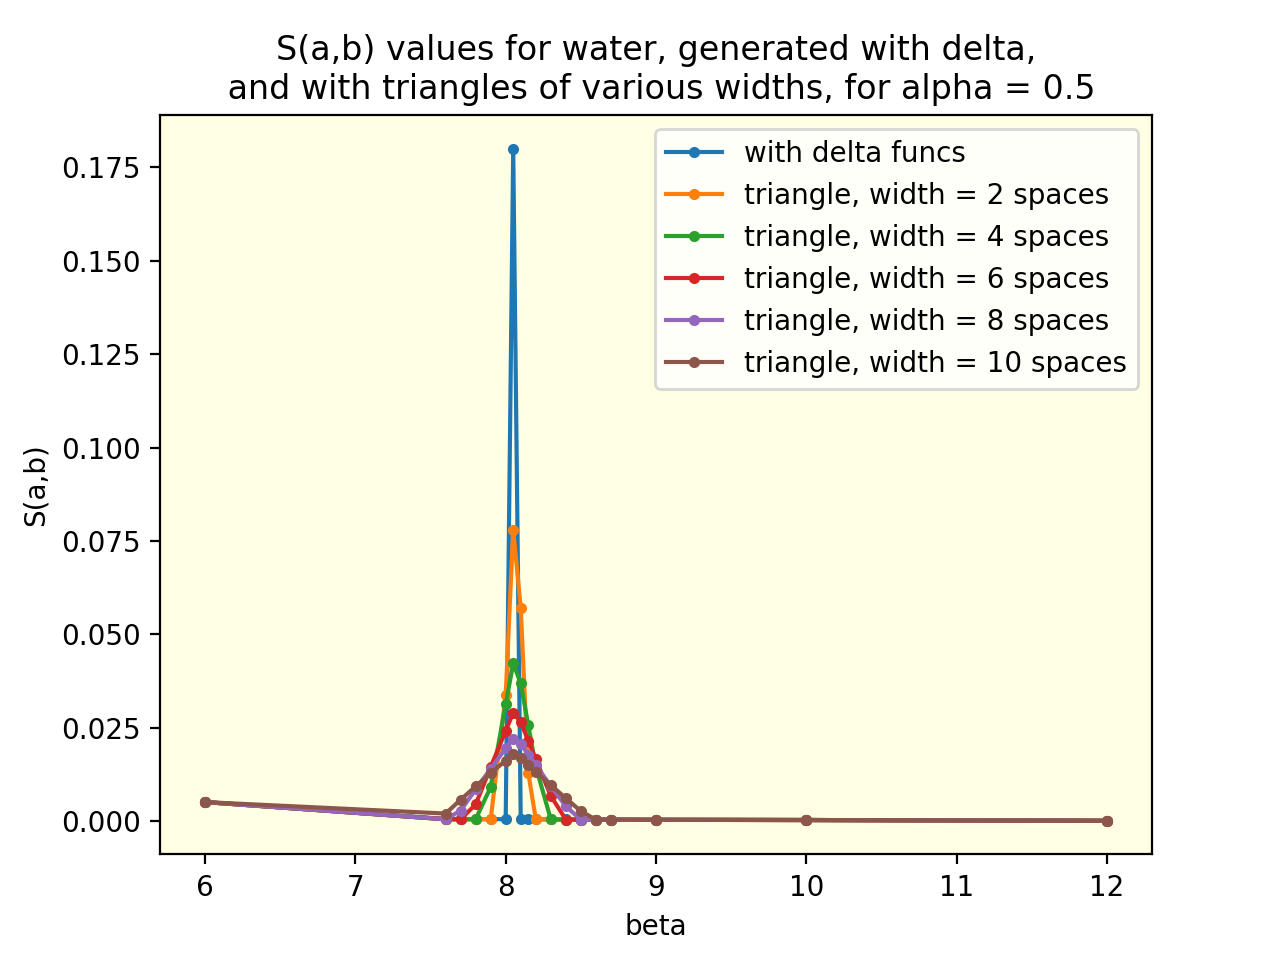
\includegraphics[scale=0.6]{diff_widths_alpha_0p5}
                \caption{}
              \label{fig:diff_widths_alpha_0p5}
              \end{center}
            \end{figure}

              
              We also look at the total error.
              \[E_{total}=\sum_{\beta}\sum_\alpha \Big|S^\delta(\alpha,\beta)-S^\triangleleft(\alpha,\beta)\Big|\]

            \begin{figure}[H]
              \begin{center}
              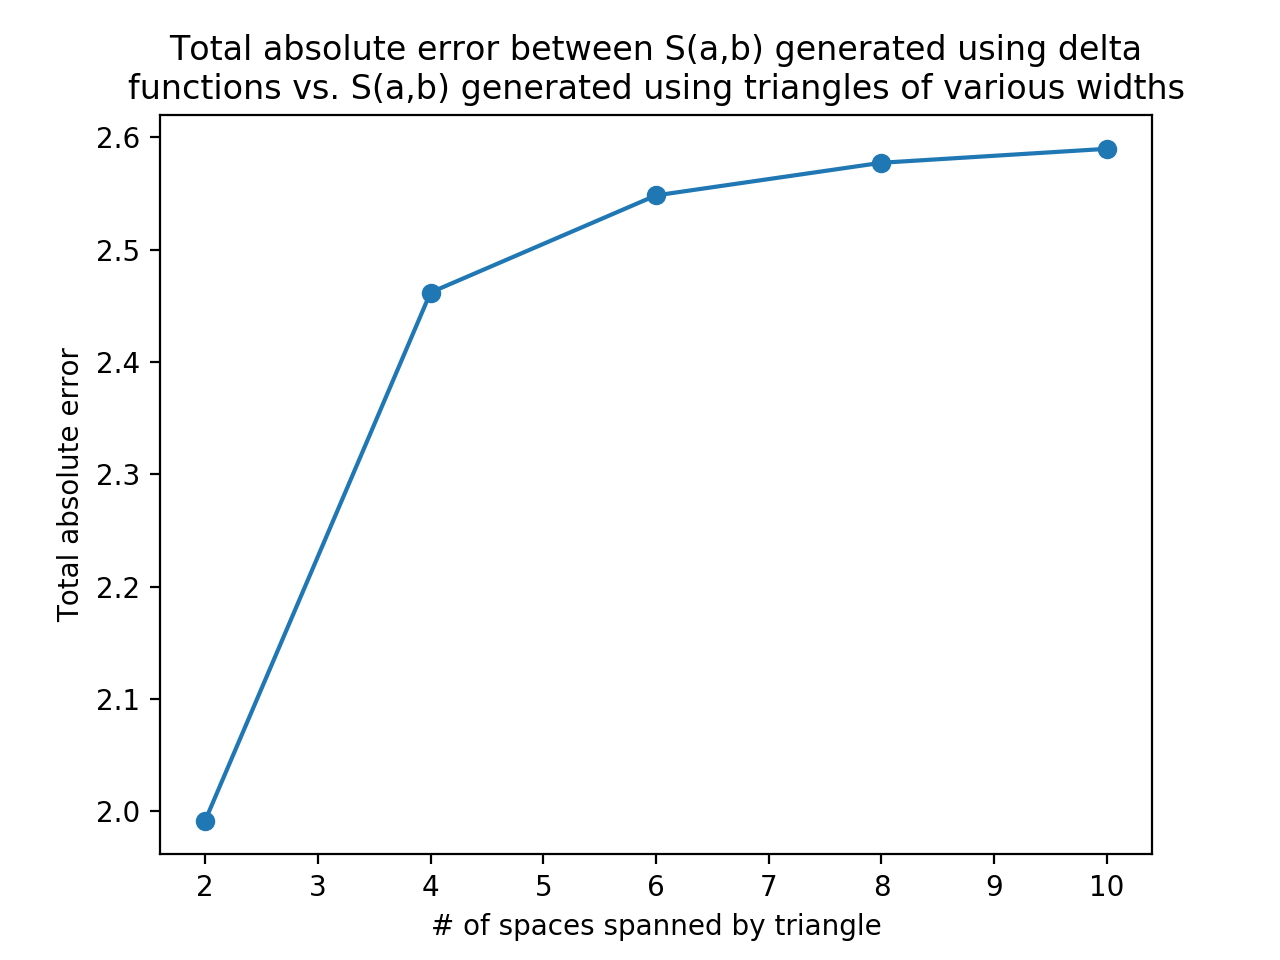
\includegraphics[scale=0.6]{diff_widths_total_error}
                \caption{Note that as the width of the triangle decreases, the total accumulated error decreases significantly.}
              \label{fig:diff_widths_total_error}
              \end{center}
            \end{figure}








            \clearpage

%  \bibliographystyle{unsrt}
%\bibliography{notes}

\end{multicols}
\end{document}
















